\documentclass[a4paper,12pt]{article}
\usepackage[margin=19mm]{geometry}
\usepackage{amsmath,amssymb,graphicx,xcolor}
\usepackage{fontspec}
\usepackage{xepersian}
\settextfont{XB Roya}
\setlatintextfont{Latin Modern Roman}
\definecolor{ink}{HTML}{173D75}
\setlength{\parindent}{0pt}
\setlength{\parskip}{5pt}
\linespread{1.12}
\newcommand{\qtitle}[2]{{\Large\bfseries\color{ink} پرسش \lr{#1}: #2}\par
{\small\textbf{وضعیت: باز.} خوانش اسلاید موقت است؛ پاسخی ثبت نشده است.}\par}
\newcommand{\sourcepage}[1]{\textbf{نشانی منبع:} نسخهٔ \lr{primary}، فایل
\lr{\texttt{04 Module.pdf}}، #1.\par}
\newcommand{\answer}{\vfill\noindent\begin{minipage}{\linewidth}
\textbf{پاسخ یا صورت مورد تأیید:}\par\vspace{12mm}\hrule\end{minipage}}
\begin{document}
{\LARGE\bfseries پرسش‌های ابهام جلسهٔ ۰۴}\par
{\large مدول‌ها — جزوهٔ جبر پیشرفتهٔ دکتر خسروی}\par
این پرونده چهار پرسش حل‌نشده را گرد می‌آورد. شمارهٔ صفحه‌ها، شمارهٔ یک‌مبنای
صفحه در فایل پی‌دی‌اف است، نه شمارهٔ دست‌نویس.
خوانش‌های موقت در اسلایدها مشخص‌اند؛ پاسخ برای بازبینی بعدی اختیاری است.
\begin{LTR}\small\texttt{sources/lectures/04 Module.pdf}\end{LTR}
\medskip\hrule\medskip

\qtitle{L04-Q01}{فرض یکانی‌بودن مدول}
\sourcepage{پایین صفحهٔ ۵ و بالای صفحهٔ ۶}
\textbf{عبارت منبع.} پس از نوشتن دو مجموعهٔ زیر، جزوه می‌گوید اگر حلقه یکدار
باشد، این دو یکی هستند:
\[
Ra=\{ra\mid r\in R\},\qquad
\langle a\rangle=\{ra+na\mid r\in R,\ n\in\mathbb Z\}.
\]
\begin{center}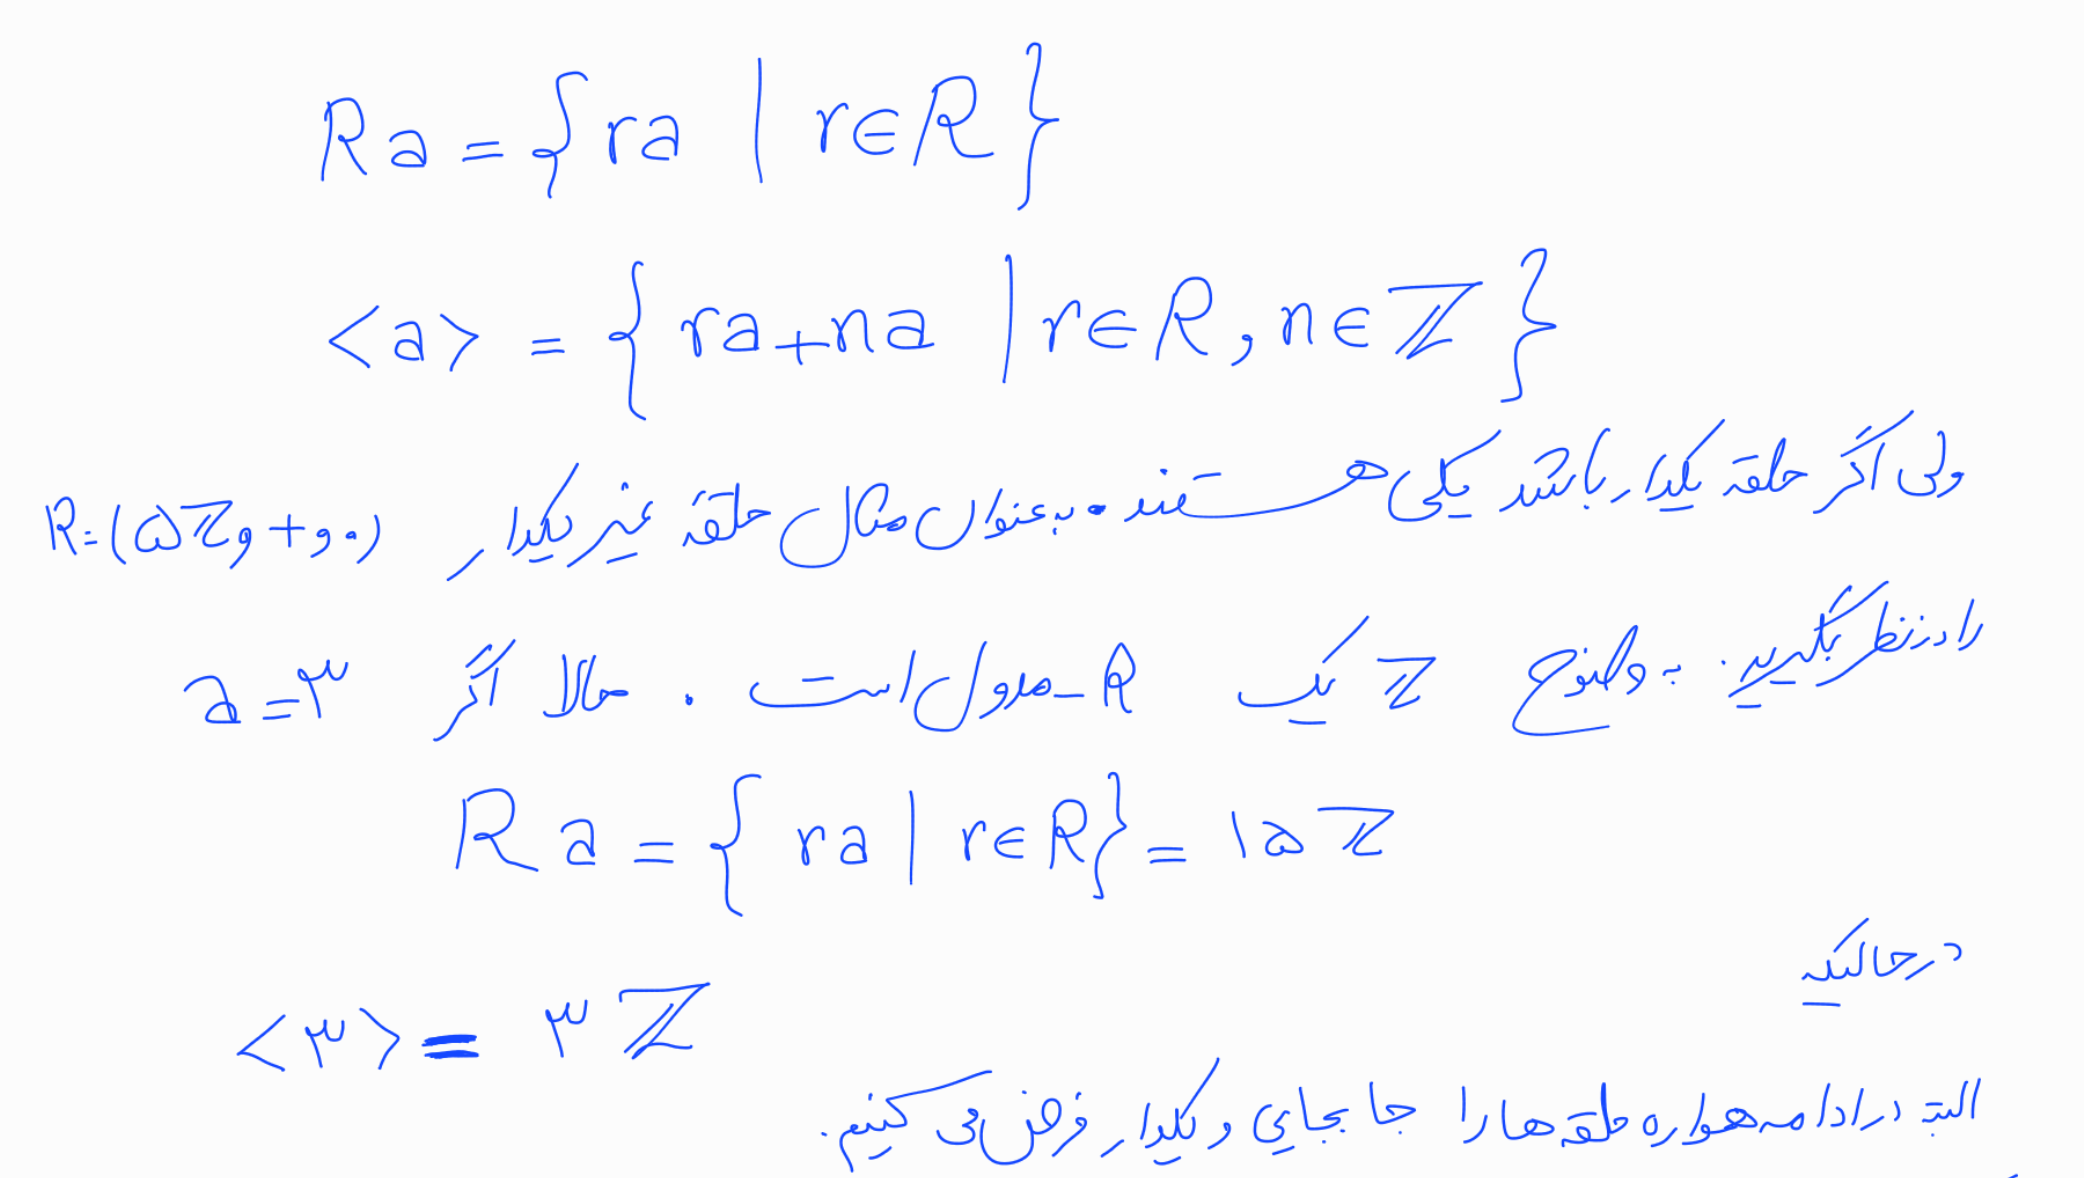
\includegraphics[width=.86\linewidth]{images/identity-assumption.png}\end{center}
\textbf{دلیل پرسش.} در تعریف اولیه، مدول لزوماً یکانی نیست و در صفحهٔ ۲
عمل صفر نیز مجاز شمرده شده است. یکداربودن حلقه به‌تنهایی شرط $1m=m$ را تضمین نمی‌کند.

\textbf{خوانش موقت اسلاید.} $M$ یکانی فرض شده و برای $R$ یکدار نوشته شده است:
\[
\langle a\rangle=Ra.
\]
\textbf{پرسش برای بازبینی.} آیا فرض یکانی‌بودن $M$ در این عبارت جزوه ضمنی است؟
\answer
\newpage

\qtitle{L04-Q02}{عضویت مولد مدول دوری}
\sourcepage{پایین صفحهٔ ۶، آغاز اثبات قضیهٔ ساختار}
\textbf{عبارت قابل مشاهده در منبع:}
\[
\exists a\in R:\qquad M=Ra.
\]
\begin{center}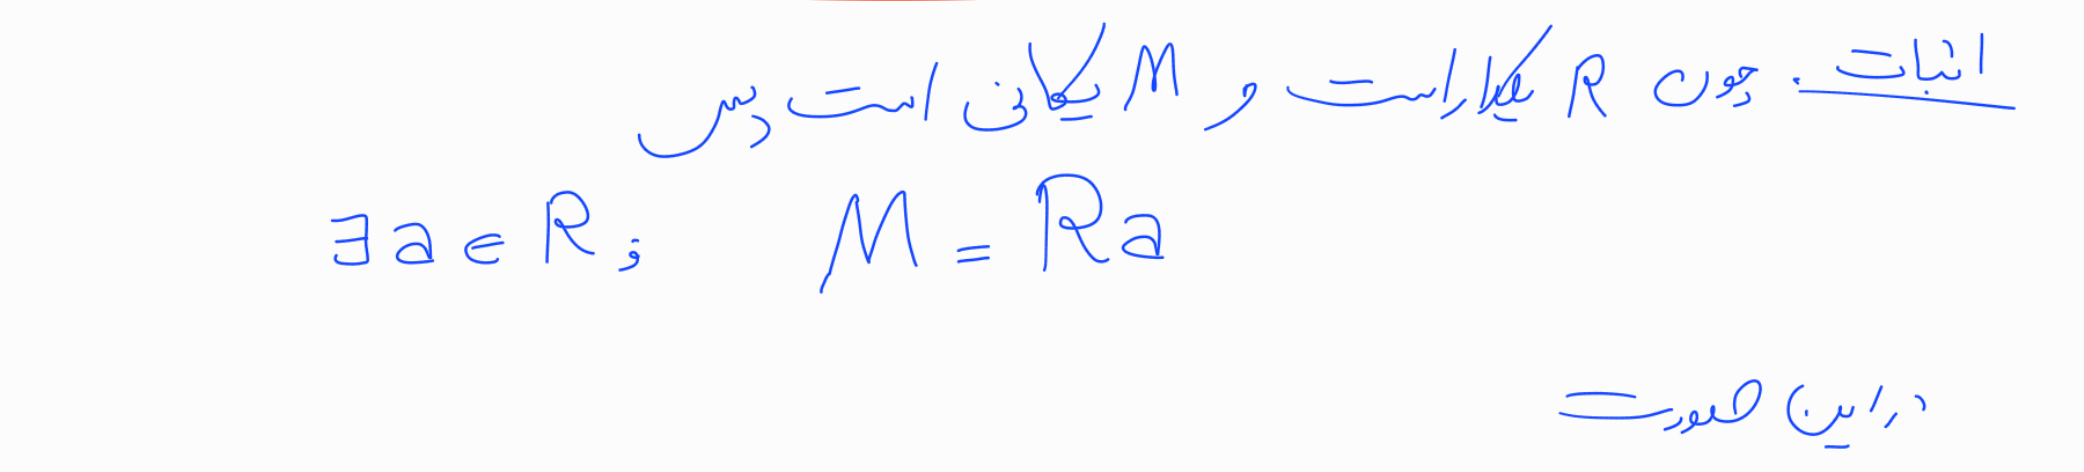
\includegraphics[width=\linewidth]{images/generator-membership.png}\end{center}
\textbf{خوانش‌های ممکن.} عبارت به‌صورت $a\in R$ نوشته شده است؛
ممکن است منظور $a\in M$ باشد.

\textbf{دلیل پرسش.} $a$ مولد مدول دلخواه $M$ است و لزومی ندارد عضوی از
خود حلقهٔ $R$ باشد.

\textbf{خوانش موقت اسلاید.} اثبات با عبارت زیر نوشته شده است:
\[
\exists a\in M:\qquad M=Ra.
\]
ادامهٔ اثبات منبع از نگاشت $r\mapsto ra$ و قضیهٔ اول یکریختی استفاده می‌کند.

\textbf{پرسش برای بازبینی.} آیا $a\in M$ خوانش درست این سطر است؟
\answer
\newpage

\qtitle{L04-Q03}{نمادگذاری نگاشت خارج‌قسمتی}
\sourcepage{میانهٔ صفحهٔ ۷، جهت عکس اثبات}
\textbf{عبارت منبع:}
\[
\varphi:R/I\longrightarrow M,\qquad r+I\longmapsto\varphi(r).
\]
\begin{center}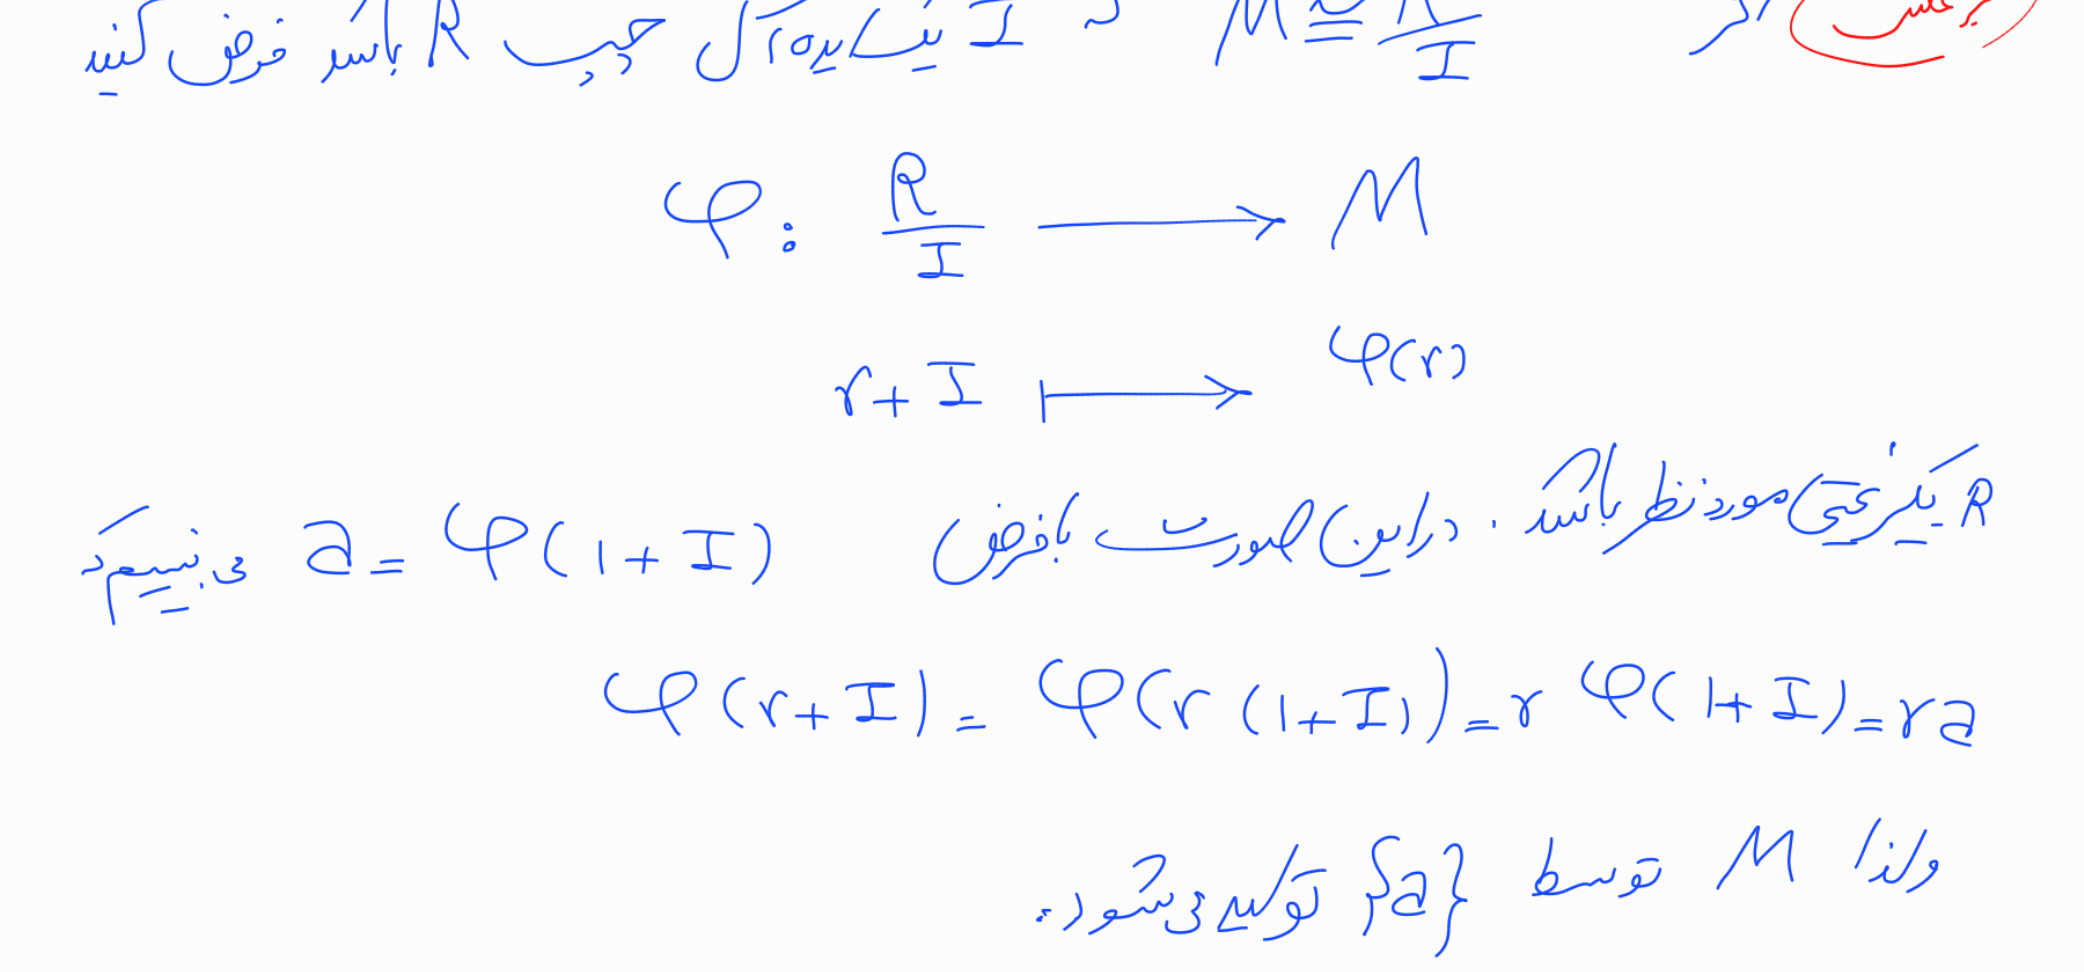
\includegraphics[width=\linewidth]{images/quotient-map.png}\end{center}
\textbf{خوانش‌های ممکن.} $\varphi(r)$ ممکن است اختصاری برای
$\varphi(r+I)$ باشد، یا نگاشتی دیگر روی $R$ در نظر گرفته شده باشد.

\textbf{دلیل پرسش.} دامنهٔ اعلام‌شده $R/I$ است، در حالی که $r$ عضوی از $R$ است.
محاسبهٔ بعدی خود جزوه از $\varphi(r+I)$ استفاده می‌کند.

\textbf{خوانش موقت اسلاید.} دامنه $R/I$ است و همهٔ ارزیابی‌ها مطابق
محاسبهٔ بعدی منبع بر همدسته نوشته شده‌اند:
\[
a=\varphi(1+I),\qquad
\varphi(r+I)=\varphi\bigl(r(1+I)\bigr)=r\varphi(1+I)=ra.
\]
\textbf{پرسش برای بازبینی.} آیا $\varphi(r)$ فقط اختصار $\varphi(r+I)$ است؟
\answer
\newpage

\qtitle{L04-Q04}{فرض تولید در معیار مجموع مستقیم}
\sourcepage{میانهٔ صفحهٔ ۹ و نتیجهٔ صفحهٔ ۱۰؛ ادامهٔ اثبات در صفحهٔ ۱۱}
\textbf{دو نکته در منبع.} در صفحهٔ ۹، زیر علامت مجموع از نماد کوچک $m_j$
استفاده شده است. در نتیجهٔ صفحهٔ ۱۰، شرط
$M=\sum_{i\in I}M_i$ در فرض‌ها ذکر نشده است.
\begin{center}
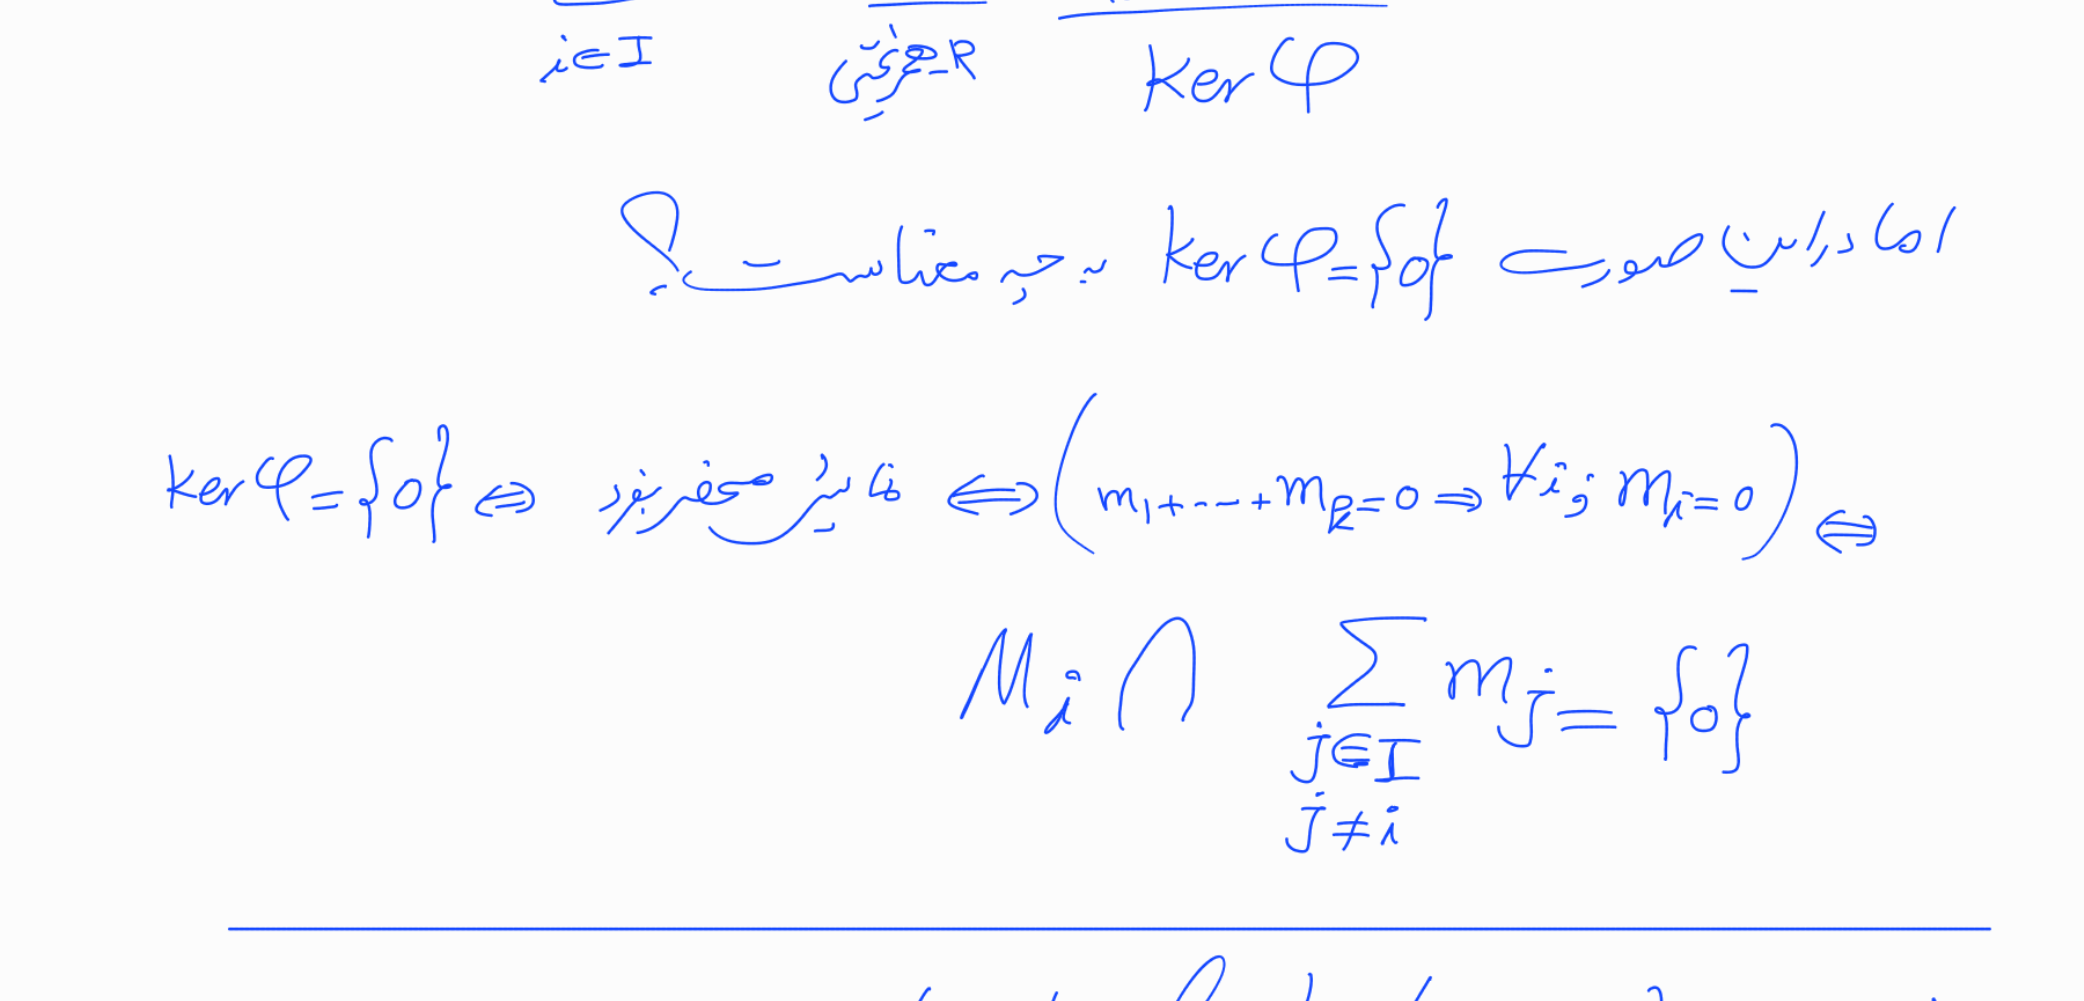
\includegraphics[width=.60\linewidth]{images/kernel-intersection.png}\\[3pt]
{\small صفحهٔ ۹}\\[5pt]
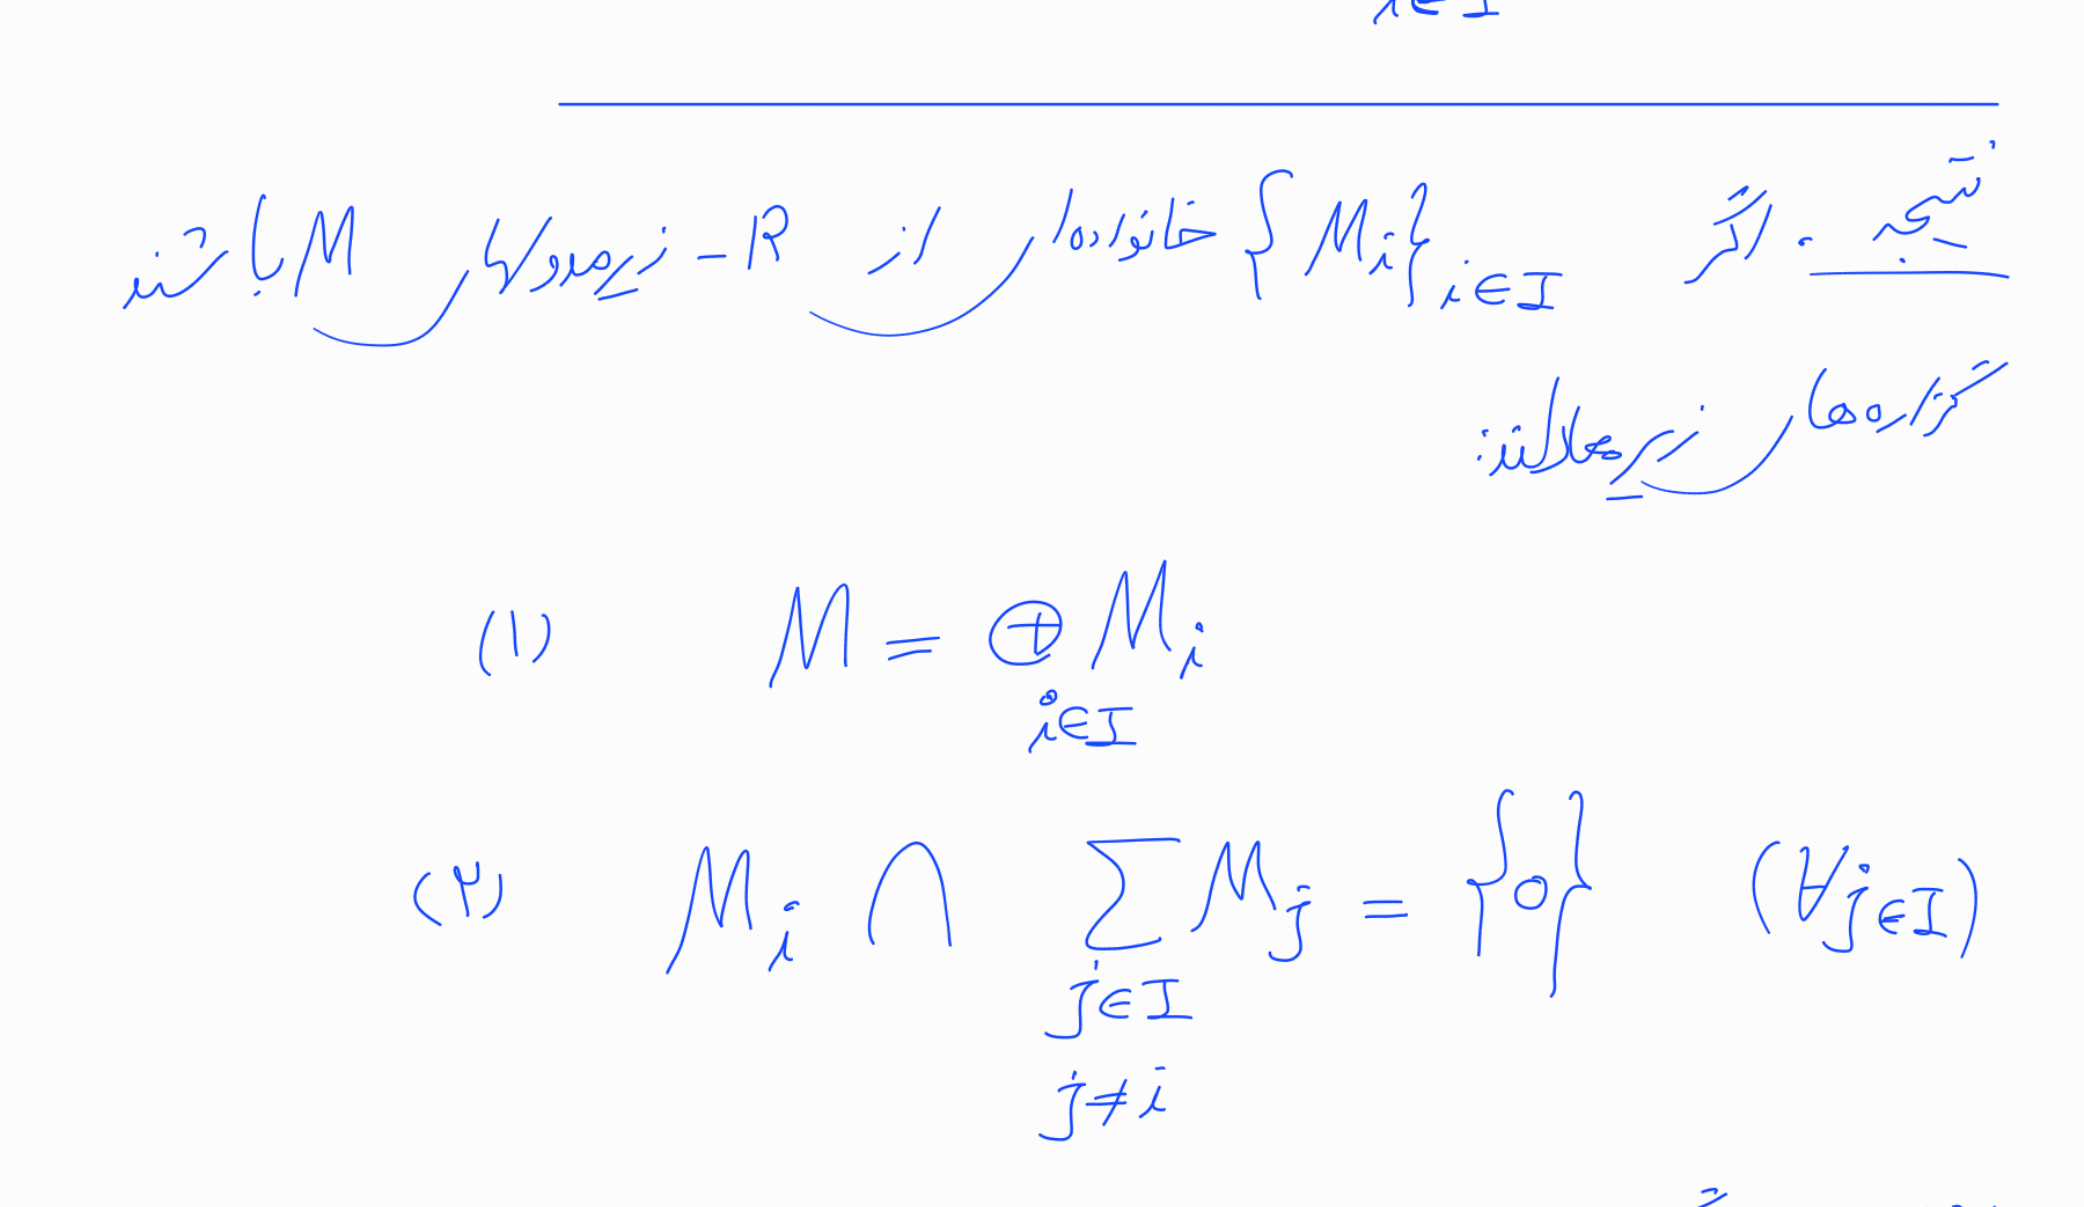
\includegraphics[width=.60\linewidth]{images/direct-sum-criterion.png}\\[3pt]
{\small صفحهٔ ۱۰}
\end{center}
\textbf{دلیل پرسش.} شرط اشتراک صفر، استقلال زیرمدول‌ها را بیان می‌کند؛
این شرط به‌تنهایی تولیدشدن تمام $M$ را تضمین نمی‌کند.

\textbf{خوانش موقت اسلاید.} نماد $M_j$ و صورت اول زیر برای بیان نتیجه و
اثبات آن به کار رفته‌اند؛ این انتخاب حل‌شدن پرسش را ادعا نمی‌کند.

\textbf{پرسش‌های بازبینی.} آیا در صفحهٔ ۹ منظور زیرمدول‌های $M_j$ است؟
کدام صورت برای نتیجه درست است؟
\begin{enumerate}
\item با فرض صریح $M=\sum_{i\in I}M_i$، مجموع مستقیم بودن $M$ با شرط
$M_i\cap\sum_{j\ne i}M_j=\{0\}$ برای هر $i$ معادل باشد.
\item نتیجه فقط دربارهٔ مجموع $\sum_{i\in I}M_i$ بیان شود، بدون ادعای برابری آن با $M$.
\end{enumerate}
\answer
\end{document}
